\documentclass[12pt]{article}
\usepackage[utf8]{inputenc}

\newenvironment{sol}[1][Solution]{\begin{trivlist}\item[\hskip\labelsep {\bfseries #1:}]}{\end{trivlist}}
\usepackage[margin=1in]{geometry} 
\usepackage{amsmath,amsthm,amssymb}
\usepackage{minted}
\usemintedstyle{vs}
\usepackage{graphicx}
\graphicspath{{./images}}
\usepackage{ amssymb }
\usepackage{times,url}  
\usepackage{hyperref}

\title{CS7381 Project 6: Verilog Code Development – MIPS ALU Controller Design }
\author{
Name: Bingying Liang \\
ID: 48999397\\  
Distance}
\date{Apr 2 2023}

\begin{document}
\maketitle
For this exercise, you will write a Verilog code program to implement the MIPS ALU Control Unit.    You will test your Control Unit module using the testbench provided in the assignment. 

Recall the following web site links for Verilog help:
\begin{itemize}
    \item \href{http://lyle.smu.edu/~manikas/CAD_tool_info.html} {http://lyle.smu.edu/~manikas/CAD\_tool\_info.html}
    \item \href{https://s2.smu.edu/~manikas/CAD_Tools/Verilog/Xcelium.html}{https://s2.smu.edu/~manikas/CAD\_Tools/Verilog/Xcelium.html}. 
\end{itemize}
In the previous Verilog assignment, you modified the code for a MIPS ALU. One of the inputs to the ALU was the ALU Control signal vector ALUctl. The ALUctl vector is output from the ALU Control Unit, and its value is based on the ALUOp signal vector from the MIPS main Control Unit and funct field of the MIPS instruction. The following table shows how these signals are mapped:
        \begin{center}
        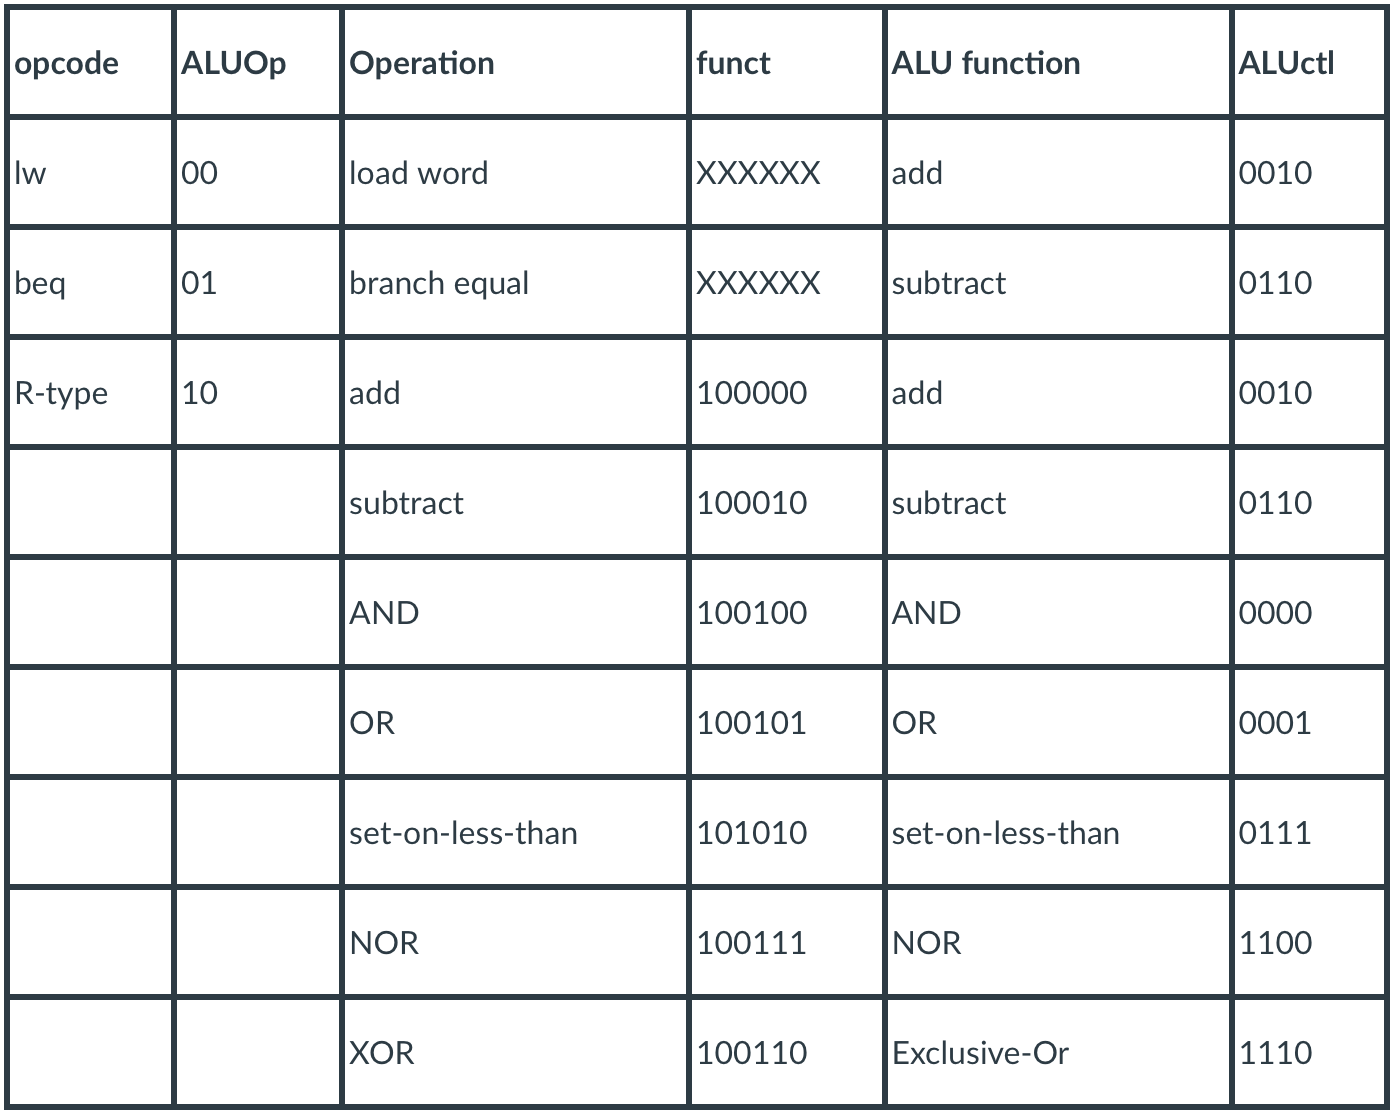
\includegraphics[width=0.76\textwidth]{p1.png}
        \end{center}

        \begin{enumerate}
            \item Please download the following Verilog file:
            \begin{enumerate}
                \item \href{https://smu.instructure.com/courses/106177/files/7254963?wrap=1}{S23\_ALU\_control\_tb.v} - the testbench for testing your ALU Control Unit
                        \begin{center}
        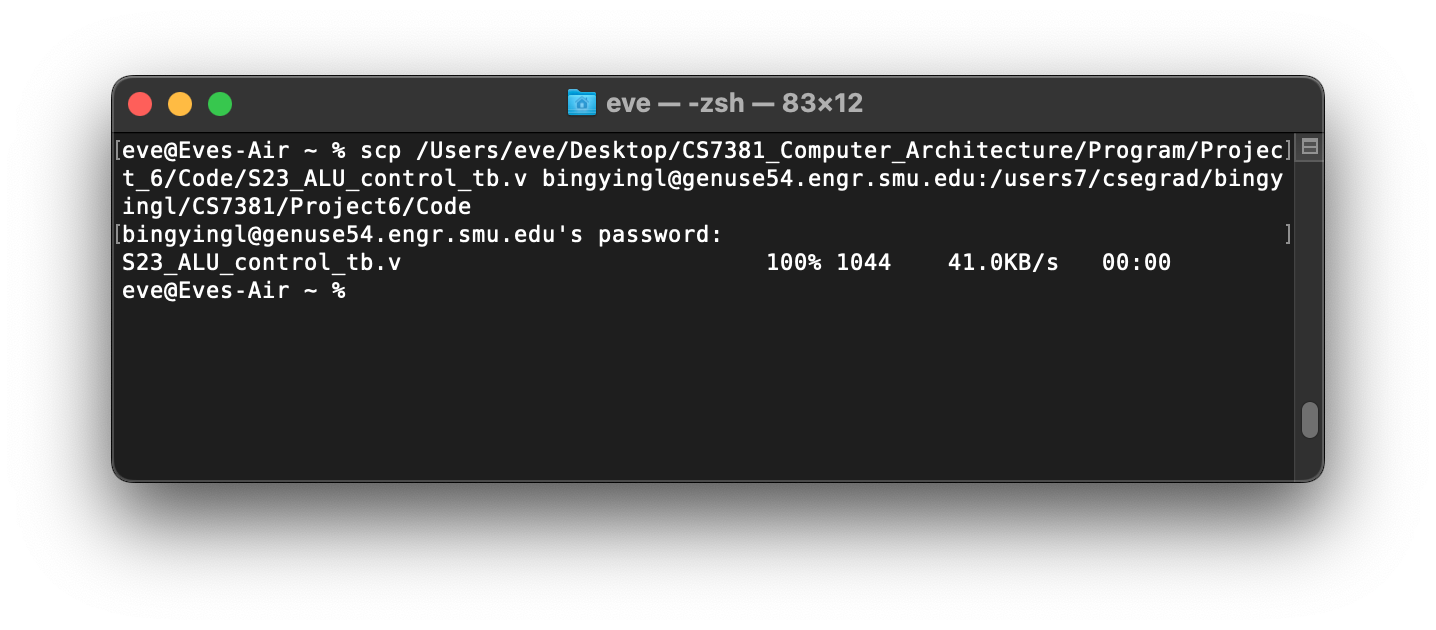
\includegraphics[width=0.9\textwidth]{p2.png}
        \end{center}
            \end{enumerate}
            \item Using the function mapping table above, design your ALU Control Unit so that it produces the correct ALU Control signal vector given the inputs ALUOp and funct.
            \begin{enumerate}
                \item Save the program as a *.v file – use the first initial of your first name and the first 4 letters of your last name, then the number 2 (to distinguish from your code for Project 5). For example, my file submission name would be tmani2.v.
                                        \begin{center}
        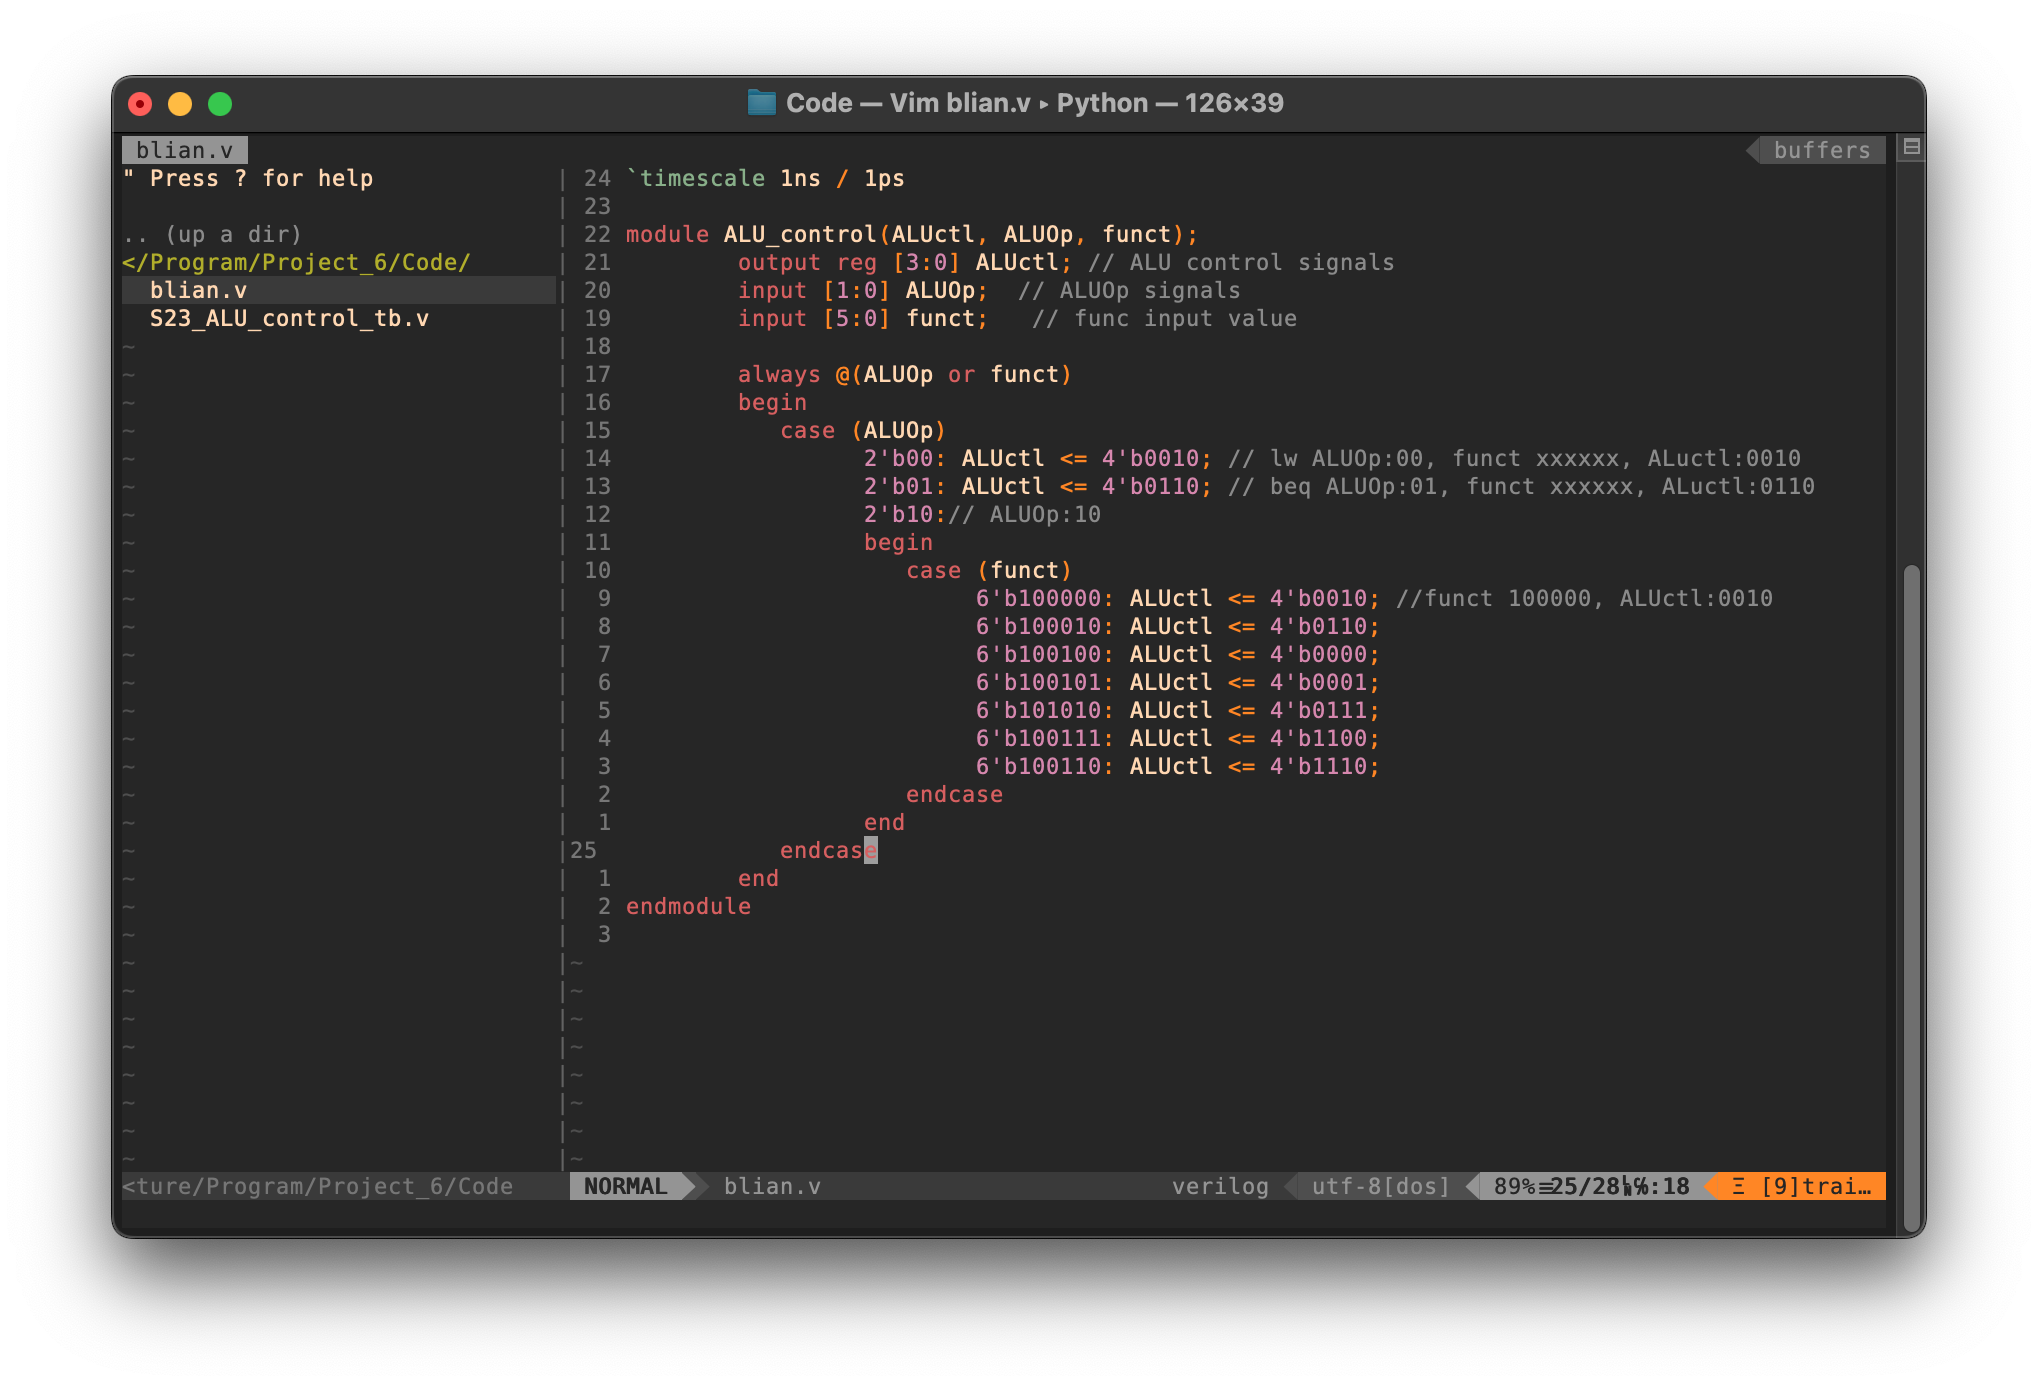
\includegraphics[width=0.9\textwidth]{p3.png}
        \end{center}
                \item Test your ALU Control Unit using the testbench provided in Step 1.
                                        \begin{center}
        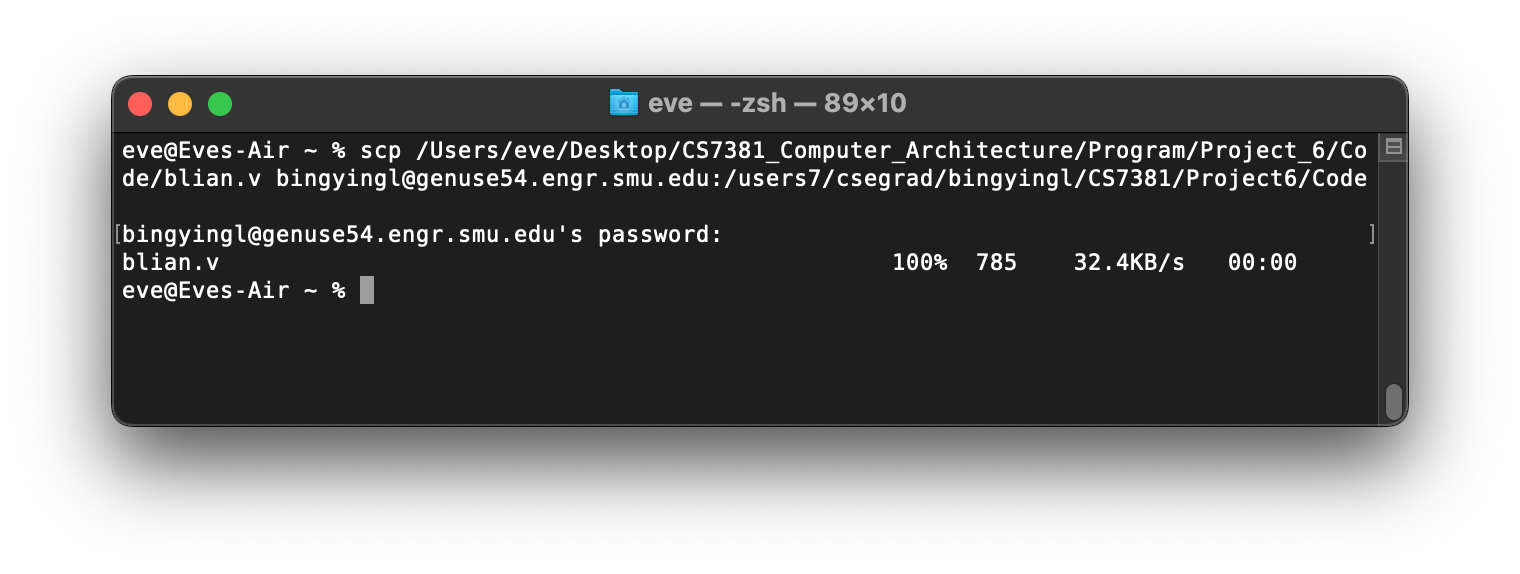
\includegraphics[width=0.9\textwidth]{p4.png}
        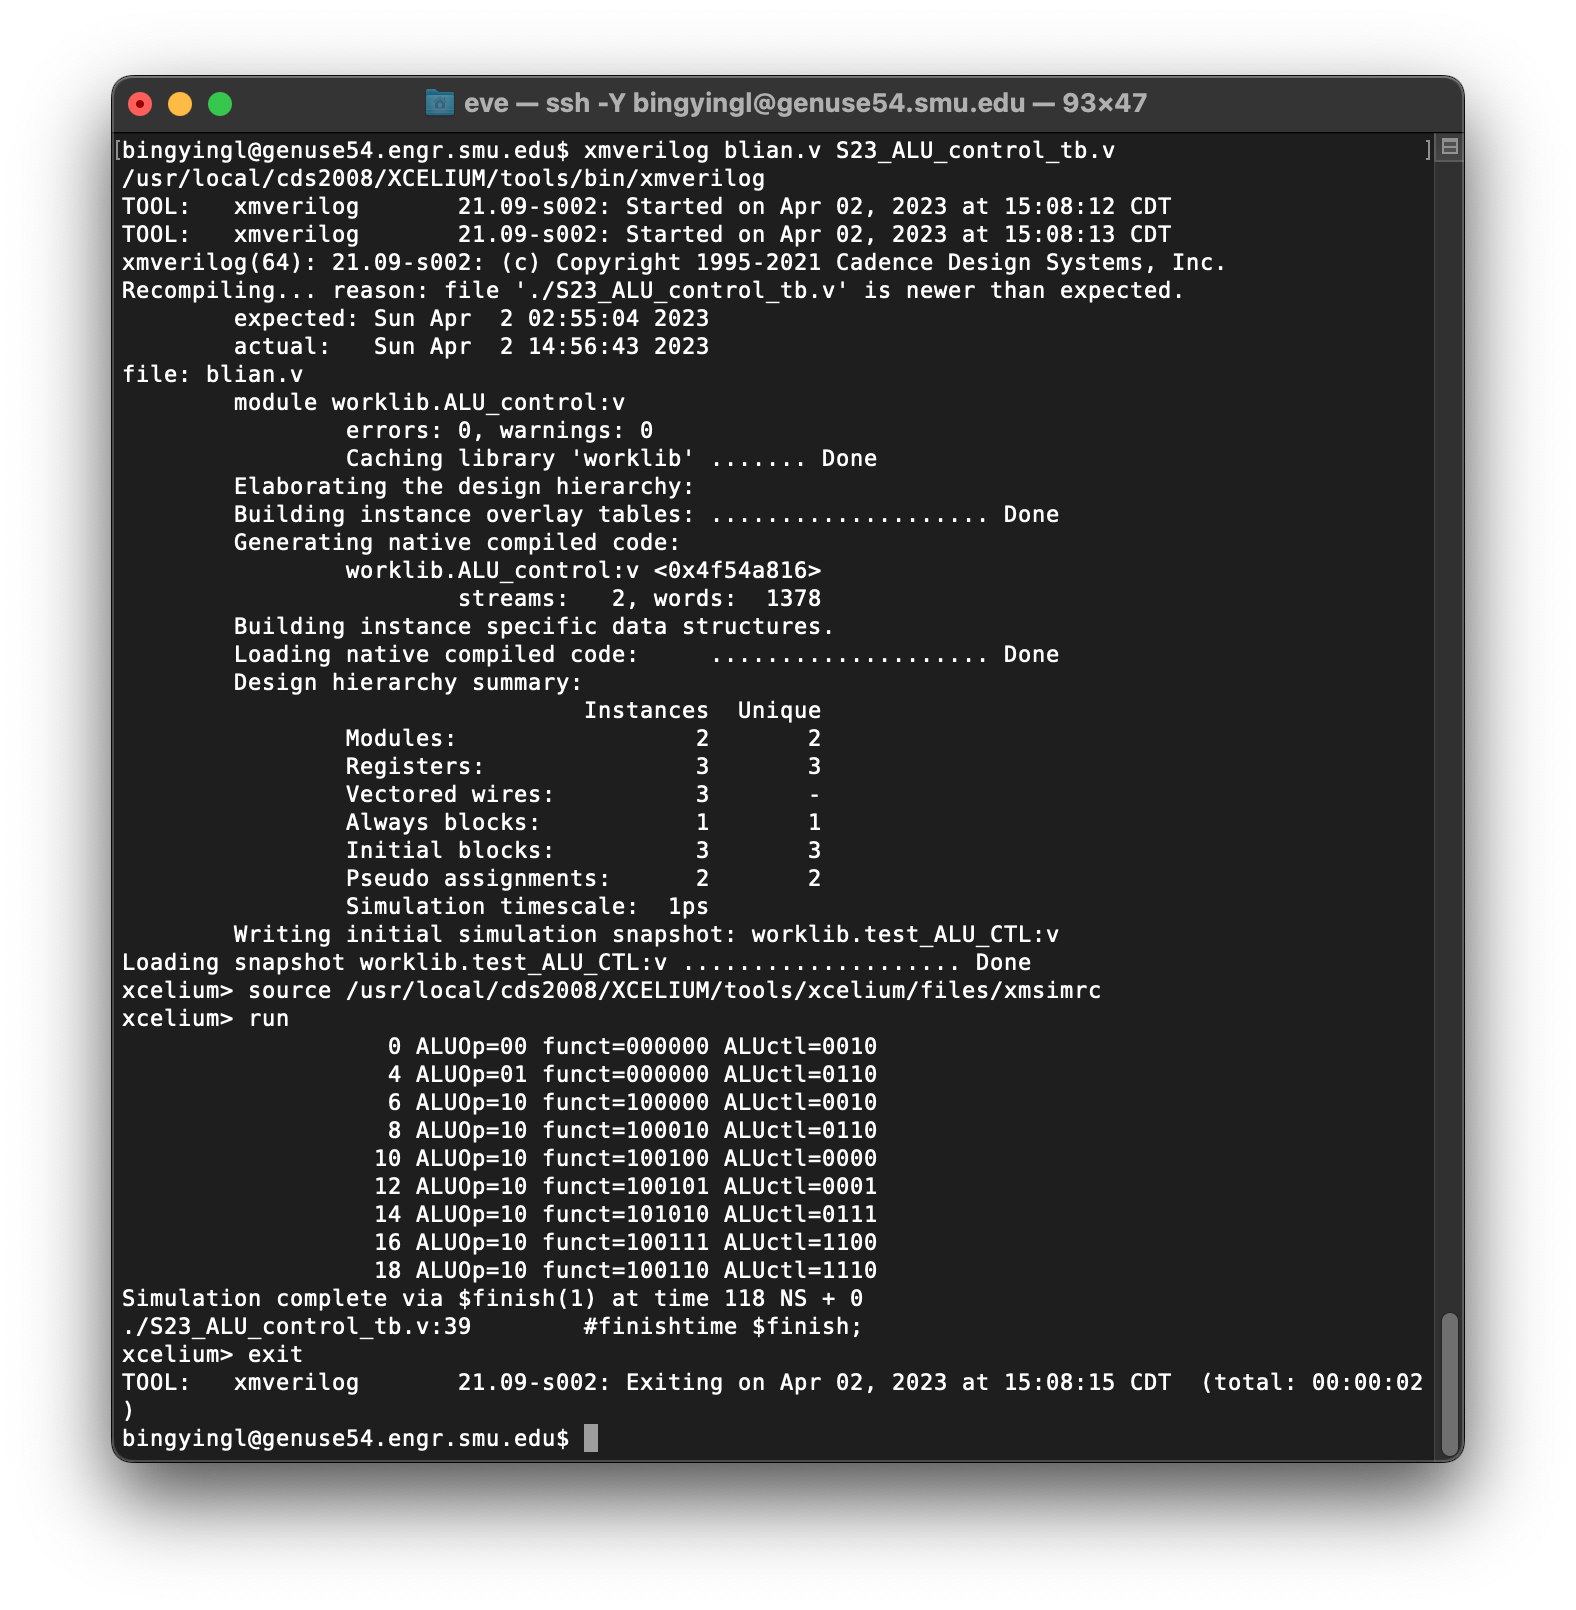
\includegraphics[width=0.9\textwidth]{p5.png}
        \end{center}
        Compare the result with testbench annotation and table they are the same and mapped correctly.
        \begin{center}
        
\includegraphics[width=0.9\textwidth]{p6.png}
        \end{center}
            \end{enumerate}
            \item Please include the following for your homework submission:
            \begin{enumerate}
                \item Your ALU Control Unit Verilog file – submit the actual *.v file so that the grader can run them.
                \begin{center}
        
\includegraphics[width=0.2\textwidth]{p7.png}
        \end{center}
                
                \item Your testbench results – this can be a copy of the results on a Word document.\\
                
                I download the result file log from the server and modify the name as blian.log
                                \begin{center}
        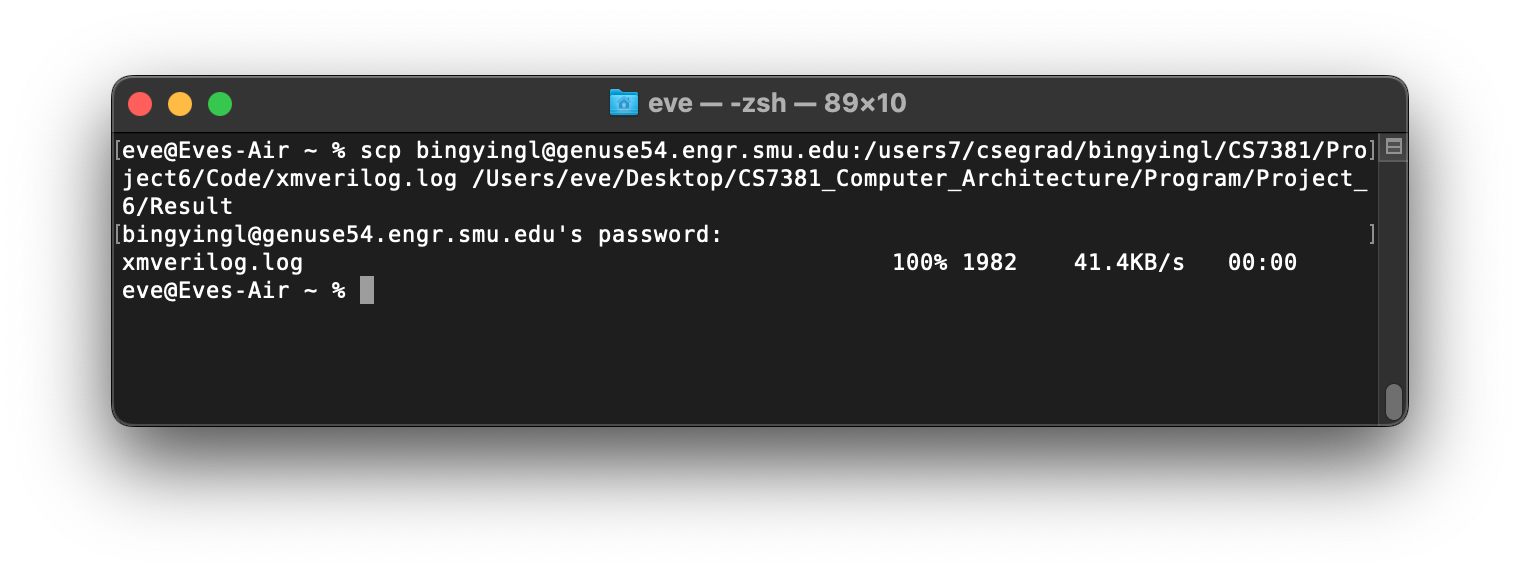
\includegraphics[width=0.9\textwidth]{p8.png}
                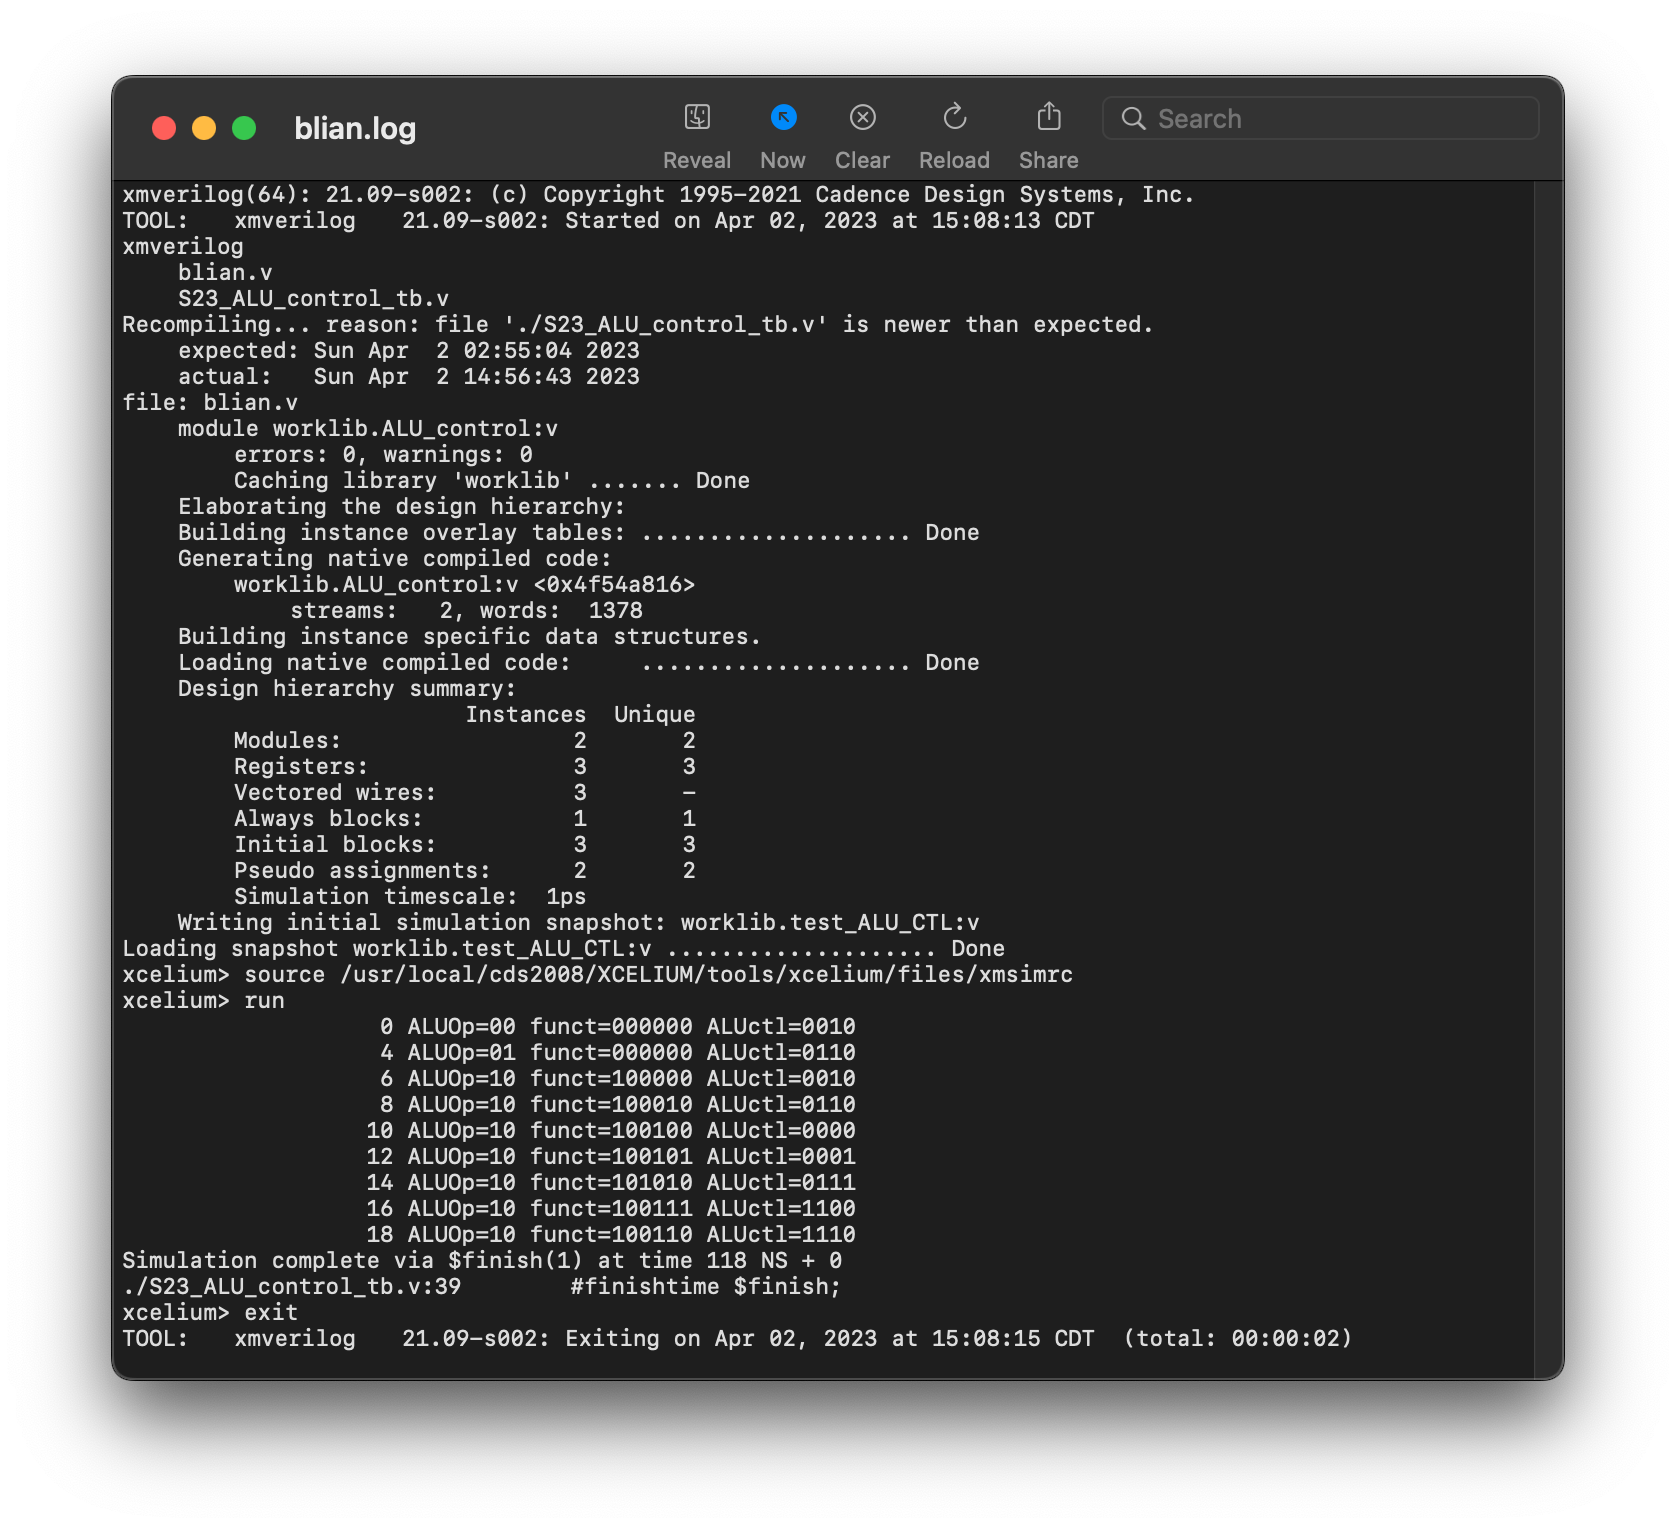
\includegraphics[width=0.9\textwidth]{p9.png}
        \end{center}
                \item PLEASE MAKE SURE THAT YOUR NAME APPEARS ON ALL SUBMITTED ITEMS FOR PROPER 
                CREDIT
            \end{enumerate}
        \end{enumerate}
\end{document}
